Komunikacja jest podstawową potrzebą człowieka, a mówienie jest jedną z najbardziej naturalnych form komunikacji poza mimiką, kontaktem wzrokowym i językiem ciała. Badanie mowy sięga jeszcze przed erą cyfrową, z legendami o urządzeniach mechanicznych, które potrafiły naśladować ludzki głos w XIII wieku \cite{introduction_springer}. Jednak rozwój przetwarzania mowy nie postępował progresywnie do 1930 roku po dwóch wynalazkach dotyczących analizy i syntezy mowy w \textit{BBC Laboratories}. Wydarzenia te są często uważane za początek epoki technologii mowy współczesnej (\ref{fig:research_lab}) \cite{introduction_speech_signals}.
\begin{figure}[h]
    \centering
    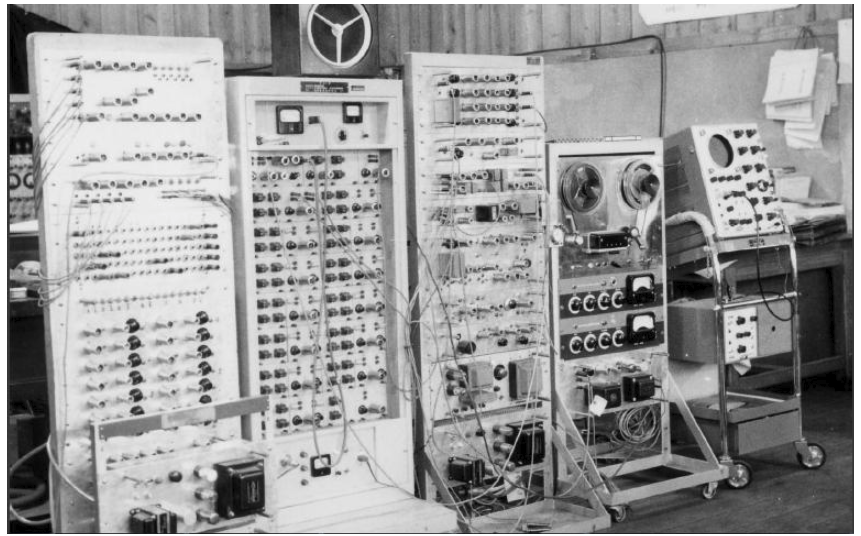
\includegraphics[width=0.5\textwidth]{images/research_lab.png}
    \caption{Japoński system rozpoznawania samogłosek z 1961 roku \cite{img_research_lab}}
    \label{fig:research_lab}
\end{figure}

Nie ma ścisłej klasyfikacji obszarów przetwarzania mowy, chociaż można wyróżnić trzy główne elementy: analiza, rozpoznanie i kodowanie mowy (\ref{fig:speech_domains}). Podstawową informacją jaką mowa dostarcza jest przekaz słowny (\textit{speech recognition}), język (\textit{language identification}) oraz informacje dot. mówcy na przykład jego płeć, emocje ect. (\textit{speaker recognition})  \cite{introduction_springer}. Praca dotyczy włącznie przekazu słownego, czyli transkrypcji źródłowych plików audio.
\begin{figure}[h]
    \centering
    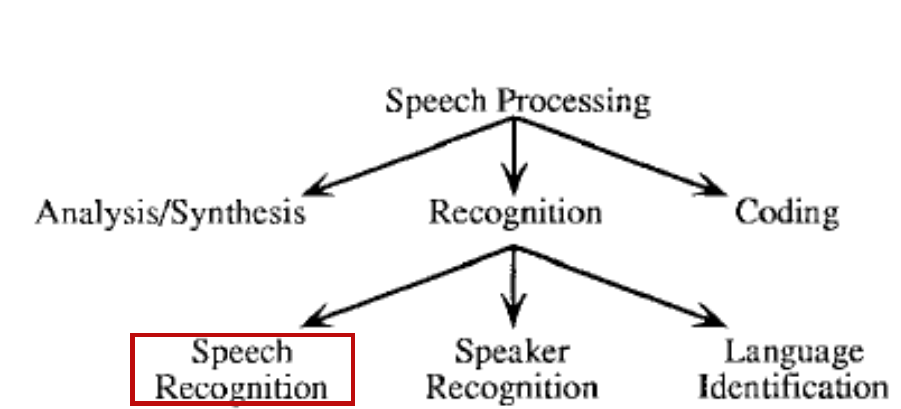
\includegraphics[width=0.5\textwidth]{images/speech_domains.png}
    \caption{Obszary przetwarzania mowy (zaadoptowane z \cite{img_speech_domains})}
    \label{fig:speech_domains}
\end{figure}

W dziedzinie rozpoznawania mowy (\textit{speech recognition}) od lat 70 XX w. szeroko stosowano ukryte modele Markova (\textit{Hidden Markov Models, \acrshort{hmm}}). Początkowo systemy rozpoznawania mowy (\textit{Automatic Speech Recognition, \acrshort{asr}}) były znacznie ograniczone. Nie potrafiły rozpoznać więcej niż kilkaset słów i często wymagały przerw pomiędzy analizowanymi sekwencjami wyrazów. Szybki rozwój komputerów w latach 90 XX w. zaowocował kilkoma złożonymi systemami bazujących na HMM. Mimo znaczącej poprawy skuteczności, systemy \acrshort{asr} nie mogły konkurować z jakością rozpoznawania mowy przez człowieka. Przełomem w \textit{speech recognition} było zastosowanie głębokich sieci neuronowych (\textit{Deep Neural Networks, \acrshort{dnn}}) na początku XXI w.

\textit{Tradycyjne} systemy rozpoznawania mowy składają się z wielu etapów, w tym: specjalistyczna ekstrakcja cech, modele akustyczne i wspomniane już modele \acrshort{hmm} (\ref{fig:schemat_rozpoznawania}). Wszystkie wymienione składowe systemu wymagają strojenia. Cała procedura stworzenia systemu jest czasochłonna i wymaga doświadczenia ekspertów. Wprowadzenie algorytmów głębokiego uczenia na początku XXI w. \cite{ds1:feature_learning, ds1:dnn_timit, ds1:accustic_modeling, ds1:dnn_hmh} poprawiło wydajność systemów poprzez ulepszanie modeli akustycznych. Mimo znaczącej poprawy skuteczności, \acrshort{dnn} odgrywały jedynie ograniczoną rolę w tradycyjnych rozwiązaniach.
\begin{figure}[h]
    \centering
    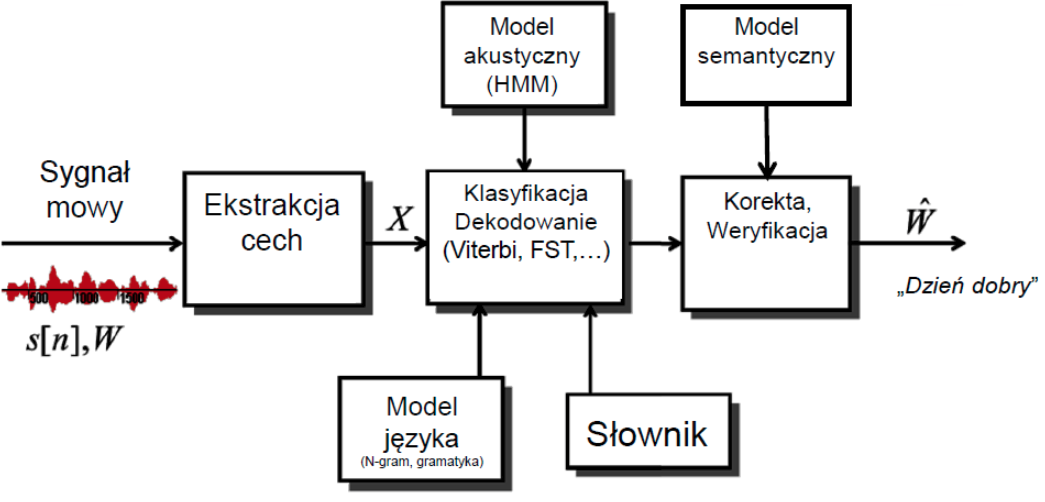
\includegraphics[width=0.6\textwidth]{images/schemat_rozpoznawania.png}
    \caption{\textit{Tradycyjny} schemat rozpoznawania mowy \cite{img_schemat_rozpoznawania}}
    \label{fig:schemat_rozpoznawania}
\end{figure}

Po raz pierwszy głęboka sieć neuronowa w całości (\textit{end-to-end}) została wykorzystana w modelu \textbf{\textit{Deep Speech}} \cite{ds1}. Zaprezentowany system nie wymaga pracochłonnego dostrajania, w tym modelowania szumu, pogłosów czy wariacji głośności. Podstawą \textit{Deep Speech} jest rekurencyjna sieć neuronowa (\textit{Recurrent Neural Network, \acrshort{rnn}}), która nie wymaga definicji fonemów. Wszystkie niezbędne informacje model pozyskuje z danych. System odniósł imponujące wyniki na szeroko studiowanym zbiorze testowym języka angielskiego \textit{Switchboard Hub5’00}.

Dekady opracowywania ręcznie wiedzy dziedzinowej ewaluowały do systemów \acrshort{asr} typu \textit{end-to-end} zastępując większość modułów jednym modelem \acrshort{dnn} \cite{ds2}. Efektywne wykorzystanie sieci \acrshort{dnn} w systemach \acrshort{asr} jest aktywnym polem badań. Częścią wspólną wszystkich modeli jest warstwa rekurencyjna (najczęściej \acrshort{lstm}) \cite{ds2:lstm1, ds2:lstm2, ds2:lstm3}. \acrlong{rnn} dobrze współpracują z warstwami konwolucyjnymi (\acrshort{cnn}), które odpowiadają za ekstrakcje cech \cite{ds2:lstm_and_conv}. Modele złożone z warstw dwukierunkowych osiągają lepsze wyniki \cite{ds2:lstm1} oraz wyposażone w mechanizm atencji \cite{ds2:attention_1, ds2:attention_2}. Wszystkie aktualnie wiodące modele rozpoznawania mowy języka angielskiego bazują na głębokim uczeniu \cite{ds3_top6,ds3_top5,ds3_top4,ds3_top3,ds3_top2,ds3_top1}. 

\section{Cel pracy}
Systemy rozpoznawanie mowy języka polskiego opierają się na \textit{tradycyjnych} rozwiązaniach \cite{pjatk_corpus}. Celem pracy jest weryfikacja skuteczności rozpoznawania mowy języka polskiego przy użyciu modeli \acrlong{dnn} typu \textit{end-to-end}. Do osiągnięcia celu i efektywnego wykorzystania zalet \acrshort{dnn} kluczowe są trzy komponenty: duży zbiór opisanych danych, architektura modelu oraz infrastruktura do efektywnego trenowania modelu \cite{ds2}. 

\section{Plan pracy}
- deep-learning
- implementacja
- eksperymenty
- wnioski
- podsumowanie / dyskusja



% Back propagation, numerical example:
% https://blog.aidangomez.ca/2016/04/17/Backpropogating-an-LSTM-A-Numerical-Example/

% EU Huge LM models:
% https://catalog.ldc.upenn.edu/LDC2009T25

% (Andrej Karpathy) The Unreasonable Effectiveness of Recurrent Neural Networks
% How RNN can decode language model
% http://karpathy.github.io/2015/05/21/rnn-effectiveness/




% -> Implementacja
%     - overview programu: schemat
%     - czym jest keras: warstwa pośrednia do backend'u - tensorflow (computation graph)
%     - przekazywanie danych do modelu: batch generation
%     - multiprocessing (fit generator): kolejka przygotowanych batchy do przetworzenia
%     - data parallelism (multi gpu model): efektywne wykorzystanie kilku GPU oraz agregacja na CPU
%     - efektywne LSTM: wykorzystanie nisko poziomowej implementacji CuDNN
%     - monitorowanie procesu trenowania: callbacks
%     - testowanie: beam search with/without lm + WER (tylko CPU support)
%     - organizacja eksperymentów: consumer
%     - rozwój: prosty sposób dodawania nowych architektur
%     - (tylko dla zwykłych rnn: seq unroll może przyspieszyć -> CuDNN ma to wbudowane?)


% -> Eksperymenty
    % -> Przygotowanie danych
    %     - dostępne zbiory danych (+benchmark ze zbioru Clarin) http://mowa.clarin-pl.eu/tools/
    %         a) Clarin 50h
    %         b) Jurisdic 450h
    %     - ekstrakcja cech: MFCC features

%     - tensorboard: wykresy dev loss (clarin)
%     - wyniki
%     - jurisdic inny learning rate
%     - okolo 20$ wykonac test na google api: https://cloud.google.com/speech-to-text/
    
% -> podsumowanie i dyskusja:
%     - przedyktowany rozdział 
%       - mało zanieczyszczone wnioski   

% *całość kodu dostępna github/rolczynski/DeepSpeech
% *mfcc features zapisywane na dysk twardy


% \section{Ograniczenia pracy}
% - ograniczenie zbioru danych
% - ograniczenie mocy obliczeniowej
% - dostosowanie infrastruktury aplikacji do ograniczeń